\documentclass[border=4pt]{standalone}
% Preámbulo común de las figuras. Cada figura es un documento standalone
% que se compila a SVG con scripts/build_figures.sh
\usepackage[utf8]{inputenc}
\usepackage{amsmath}
\usepackage{tikz}
\usepackage[american, siunitx]{circuitikz}
\usetikzlibrary{arrows.meta,calc,decorations.pathmorphing,patterns}
\tikzset{
  >={Stealth[length=2.2mm]},
  eje/.style={->, thin},
  hilo/.style={thick},
}
% Paleta común: tonos medios legibles sobre fondo claro
\definecolor{azul}{RGB}{31,94,168}
\definecolor{rojo}{RGB}{192,57,43}
\definecolor{verde}{RGB}{39,128,73}
\definecolor{naranja}{RGB}{211,120,30}
\definecolor{morado}{RGB}{125,60,152}

\begin{document}
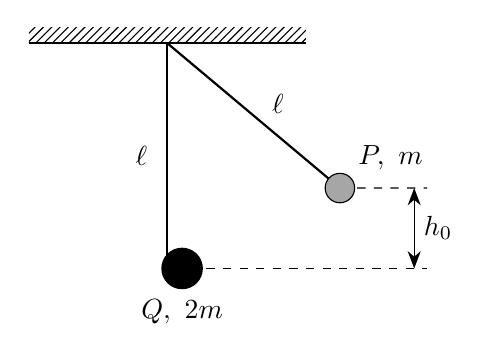
\begin{tikzpicture}[scale=1.1]
  \fill[pattern=north east lines] (-1.6,0) rectangle (1.6,0.18);
  \draw[thick] (-1.6,0) -- (1.6,0);
  \coordinate (O) at (0,0);
  \coordinate (Q) at (0,-2.6);
  \coordinate (P) at ({2.6*sin(50)},{-2.6*cos(50)});
  \draw[hilo] (O) -- (Q);
  \draw[hilo] (O) -- (P);
  \fill[gray!70] (P) circle (0.17);
  \draw (P) circle (0.17);
  \fill[black] (0.17,-2.6) circle (0.24);
  \node[above right] at ($(P)+(0.1,0.1)$) {$P,\ m$};
  \node[below] at (0.17,-2.85) {$Q,\ 2m$};
  \node[left] at (-0.12,-1.3) {$\ell$};
  \node[above right] at ($(O)!0.55!(P)$) {$\ell$};
  \draw[dashed, thin] ($(P)+(0.2,0)$) -- (3.0,{-2.6*cos(50)});
  \draw[dashed, thin] (0.45,-2.6) -- (3.0,-2.6);
  \draw[<->] (2.85,{-2.6*cos(50)}) -- node[right]{$h_0$} (2.85,-2.6);
\end{tikzpicture}
\end{document}
